\chapter{User Documentation}
\label{chap:user}

This chapter describes how the suggester should be used. It is divided into 2 parts:
\begin{itemize}
    \item User guide \ref{user_guide} – usage described from the end user point of view.
    \item Administrator guide \ref{administrator_guide} – describes how to modify suggester configuration.
\end{itemize}

\section{User guide}
\label{user_guide}
When the OpenGrok main web page is opened then the user sees something similar to the figure \ref{opengrok_main}.
When user types text into one of the search fields, suggestions are shown as can be seen on \ref{suggestions_pic}.

\begin{figure}[htbp]
    \centering
    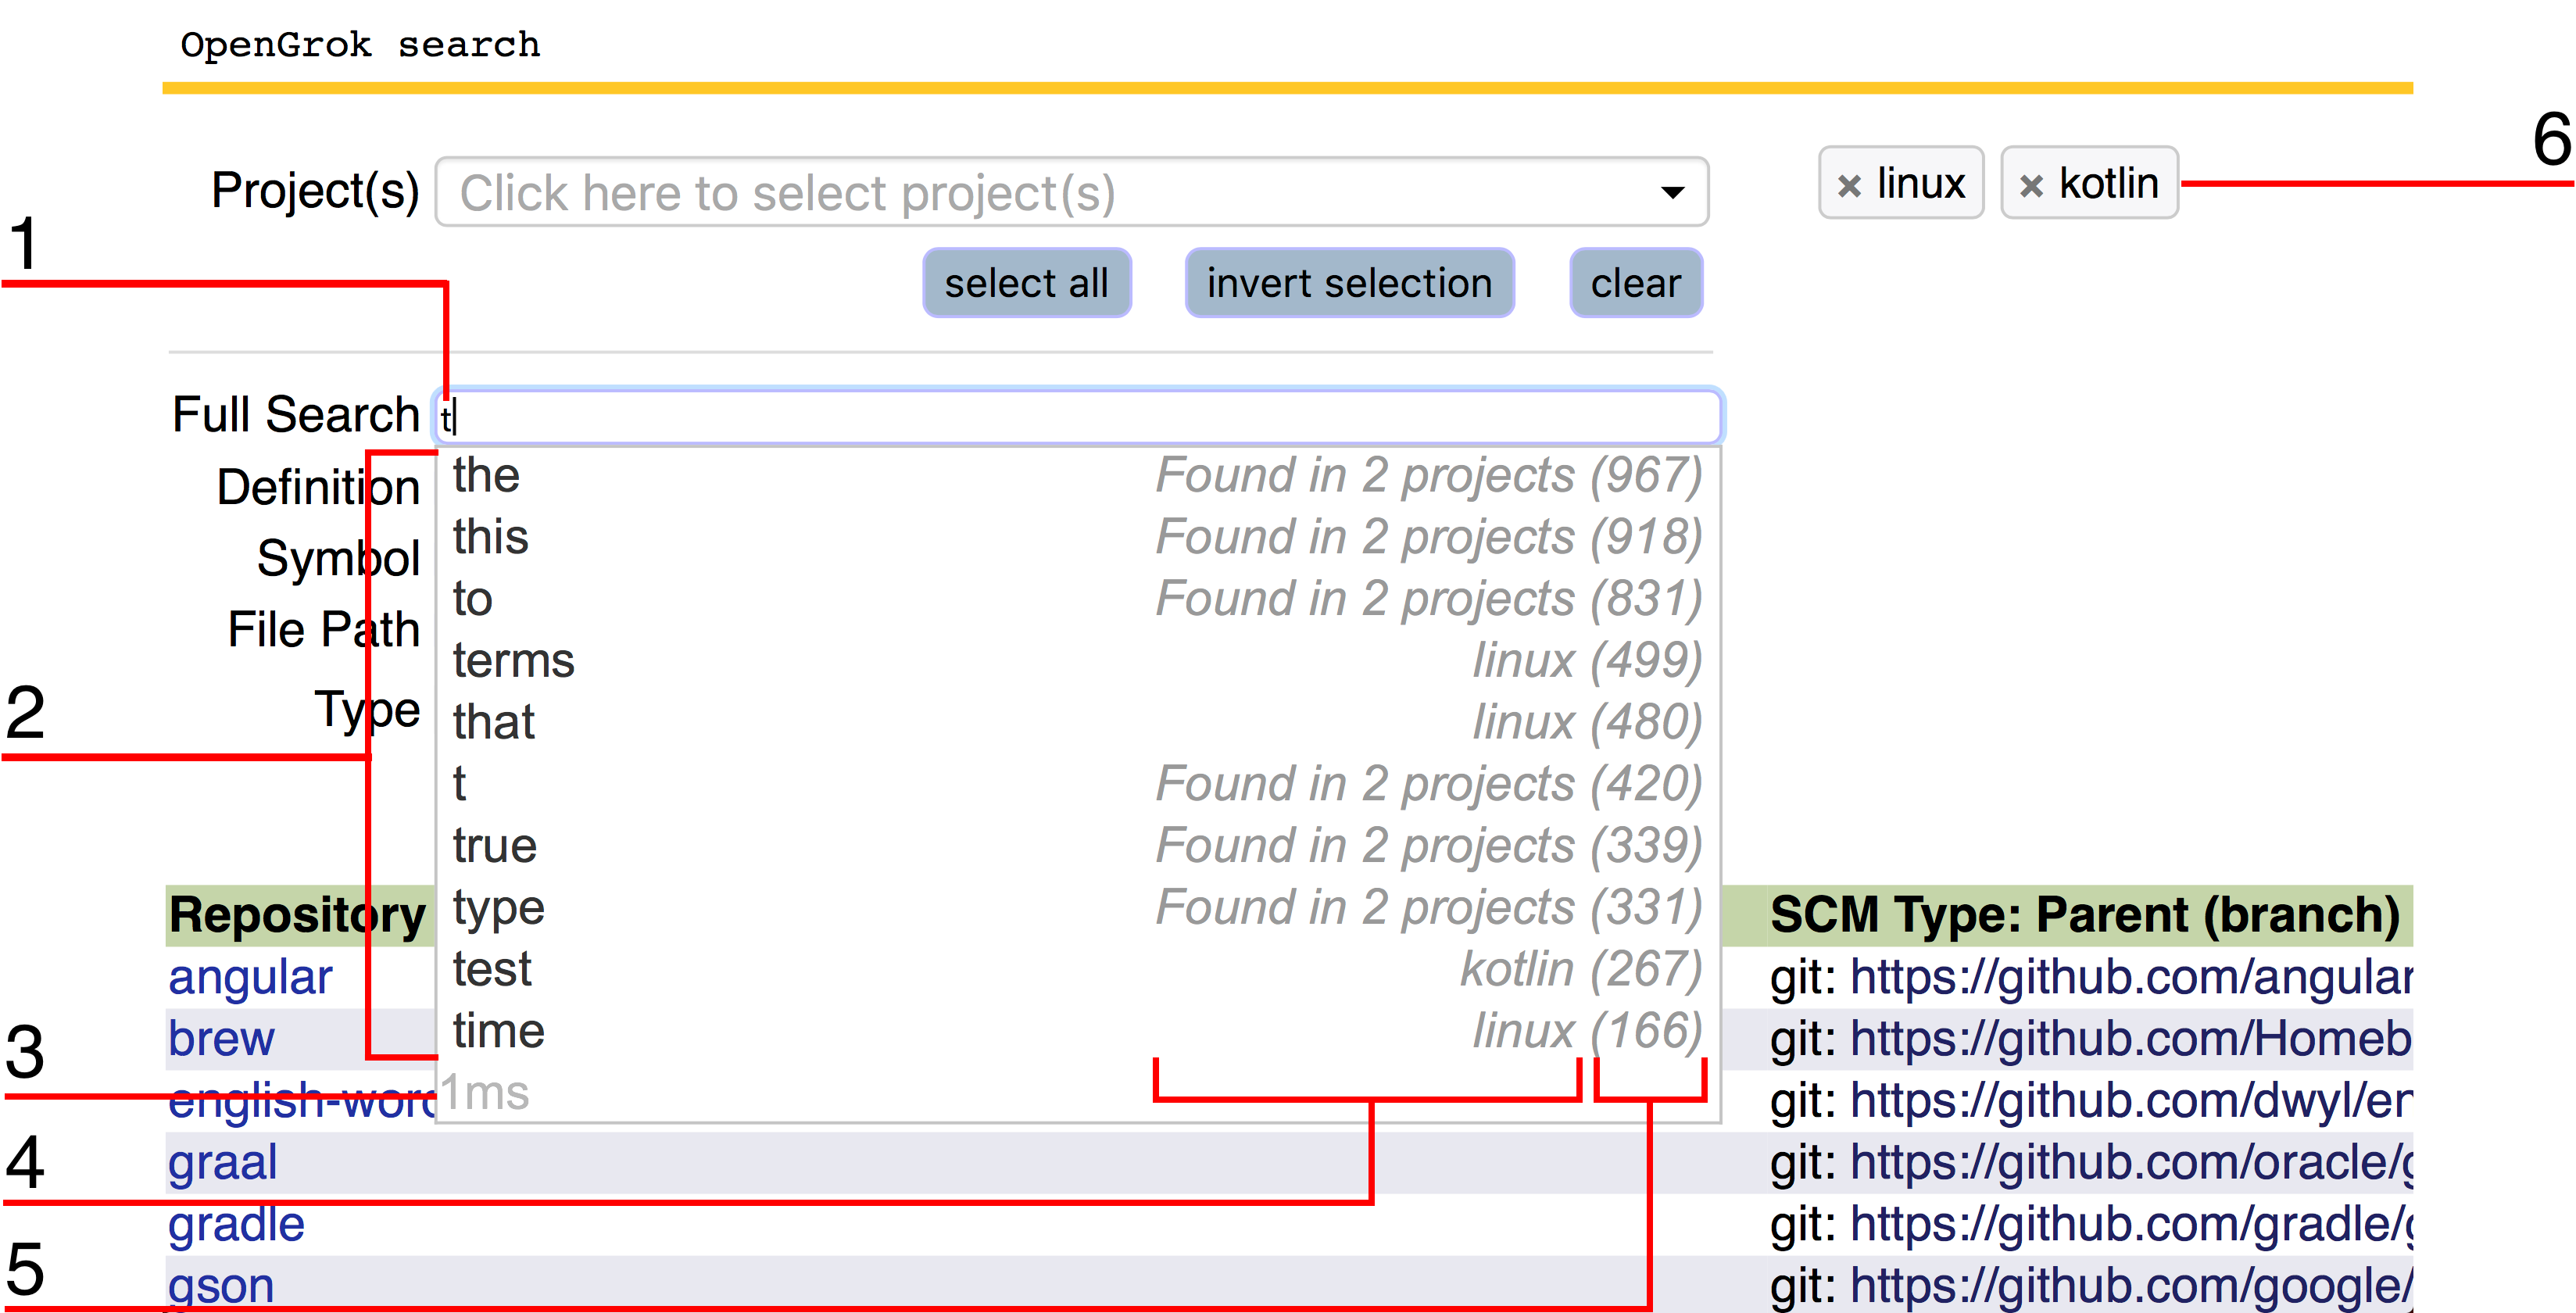
\includegraphics[width=145mm]{../img/suggestions_pic.png}
    \caption{Suggestions example}
    \label{suggestions_pic}
\end{figure}

The numbers in the picture \ref{suggestions_pic} represent:
\begin{enumerate}
    \item Typed value into the search field. In this case letter \textit{t}.
    \item List of suggestions.
    \item Time it took to generate the suggestions. (Optional.)
    \item In which projects was the term found. (Optional.)
    \item Score of the terms. (Optional.)
    \item Projects for which suggestions are shown.
\end{enumerate}

\subsection{Selecting the suggestions}
Suggestions can be navigated by using:
\begin {itemize}
    \item \textbf{Keyboard} – the suggestion can be focused by using up $\uparrow$ and down $\downarrow$ arrow keys.
    The suggestion can be selected by pressing the \textit{enter} (carriage return) or \textit{tab} key.
    The suggestions can also be closed by pressing the \textit{esc} key.
    \item \textbf{Mouse} – by hovering over the suggestion it is focused. By clicking on the suggestion it
    is selected.
\end{itemize}

\subsubsection{Focused suggestion}
If suggestion is focused then its background color is changed to \textit{blue} and the text of the field shows the result
value as if this suggestion would be selected. It looks like the figure \ref{suggestion_focused}.

\begin{figure}[htbp]
    \centering
    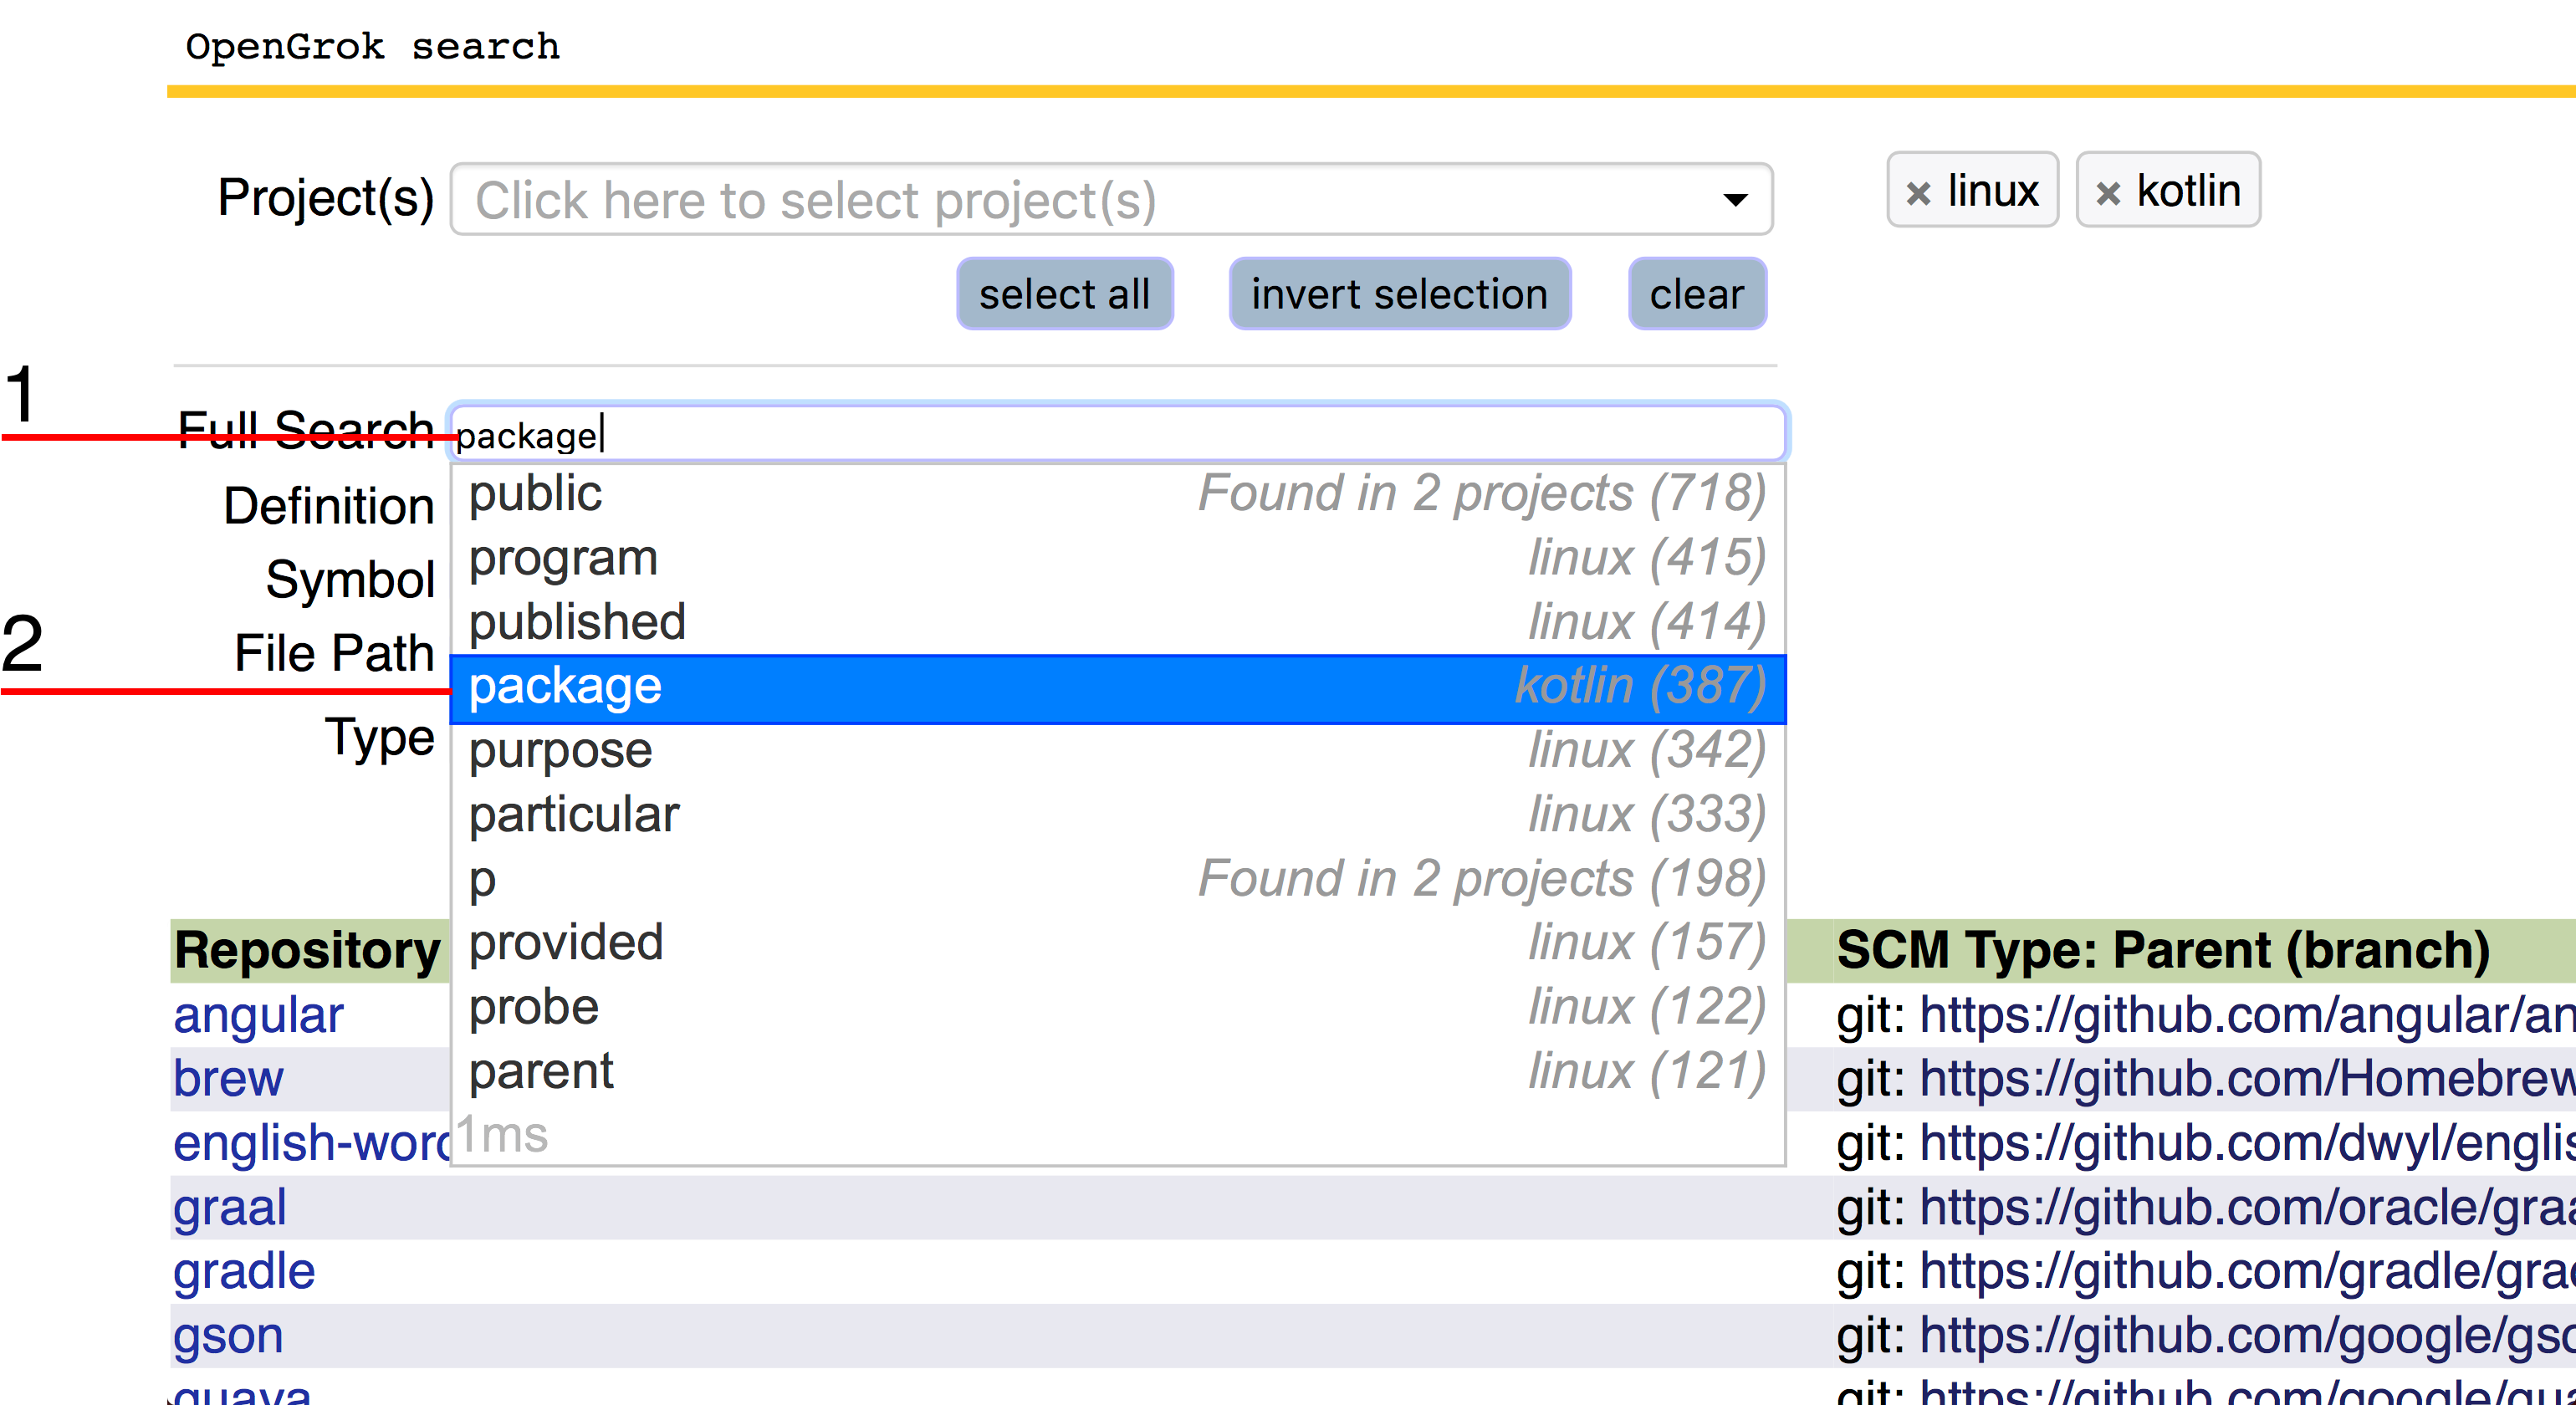
\includegraphics[width=145mm]{../img/suggestions_focused.png}
    \caption{Suggestion focused}
    \label{suggestion_focused}
\end{figure}

The numbers in the figure \ref{suggestion_focused} represent:
\begin{enumerate}
    \item The field already contains value \textit{package} even though only the prefix \textit{p} is actually written.
    \item Focused suggestion.
\end{enumerate}

\subsubsection{Errors}
It might be a common occurrence that users type an invalid query. For instance, \textit{)} is missing at the end of
the query \textit{(test}. Therefore, the user is notified if the Lucene cannot parse the query or some other
error occurs. This case is pictured in the figure \ref{suggestions_error}.

\begin{figure}[htbp]
    \centering
    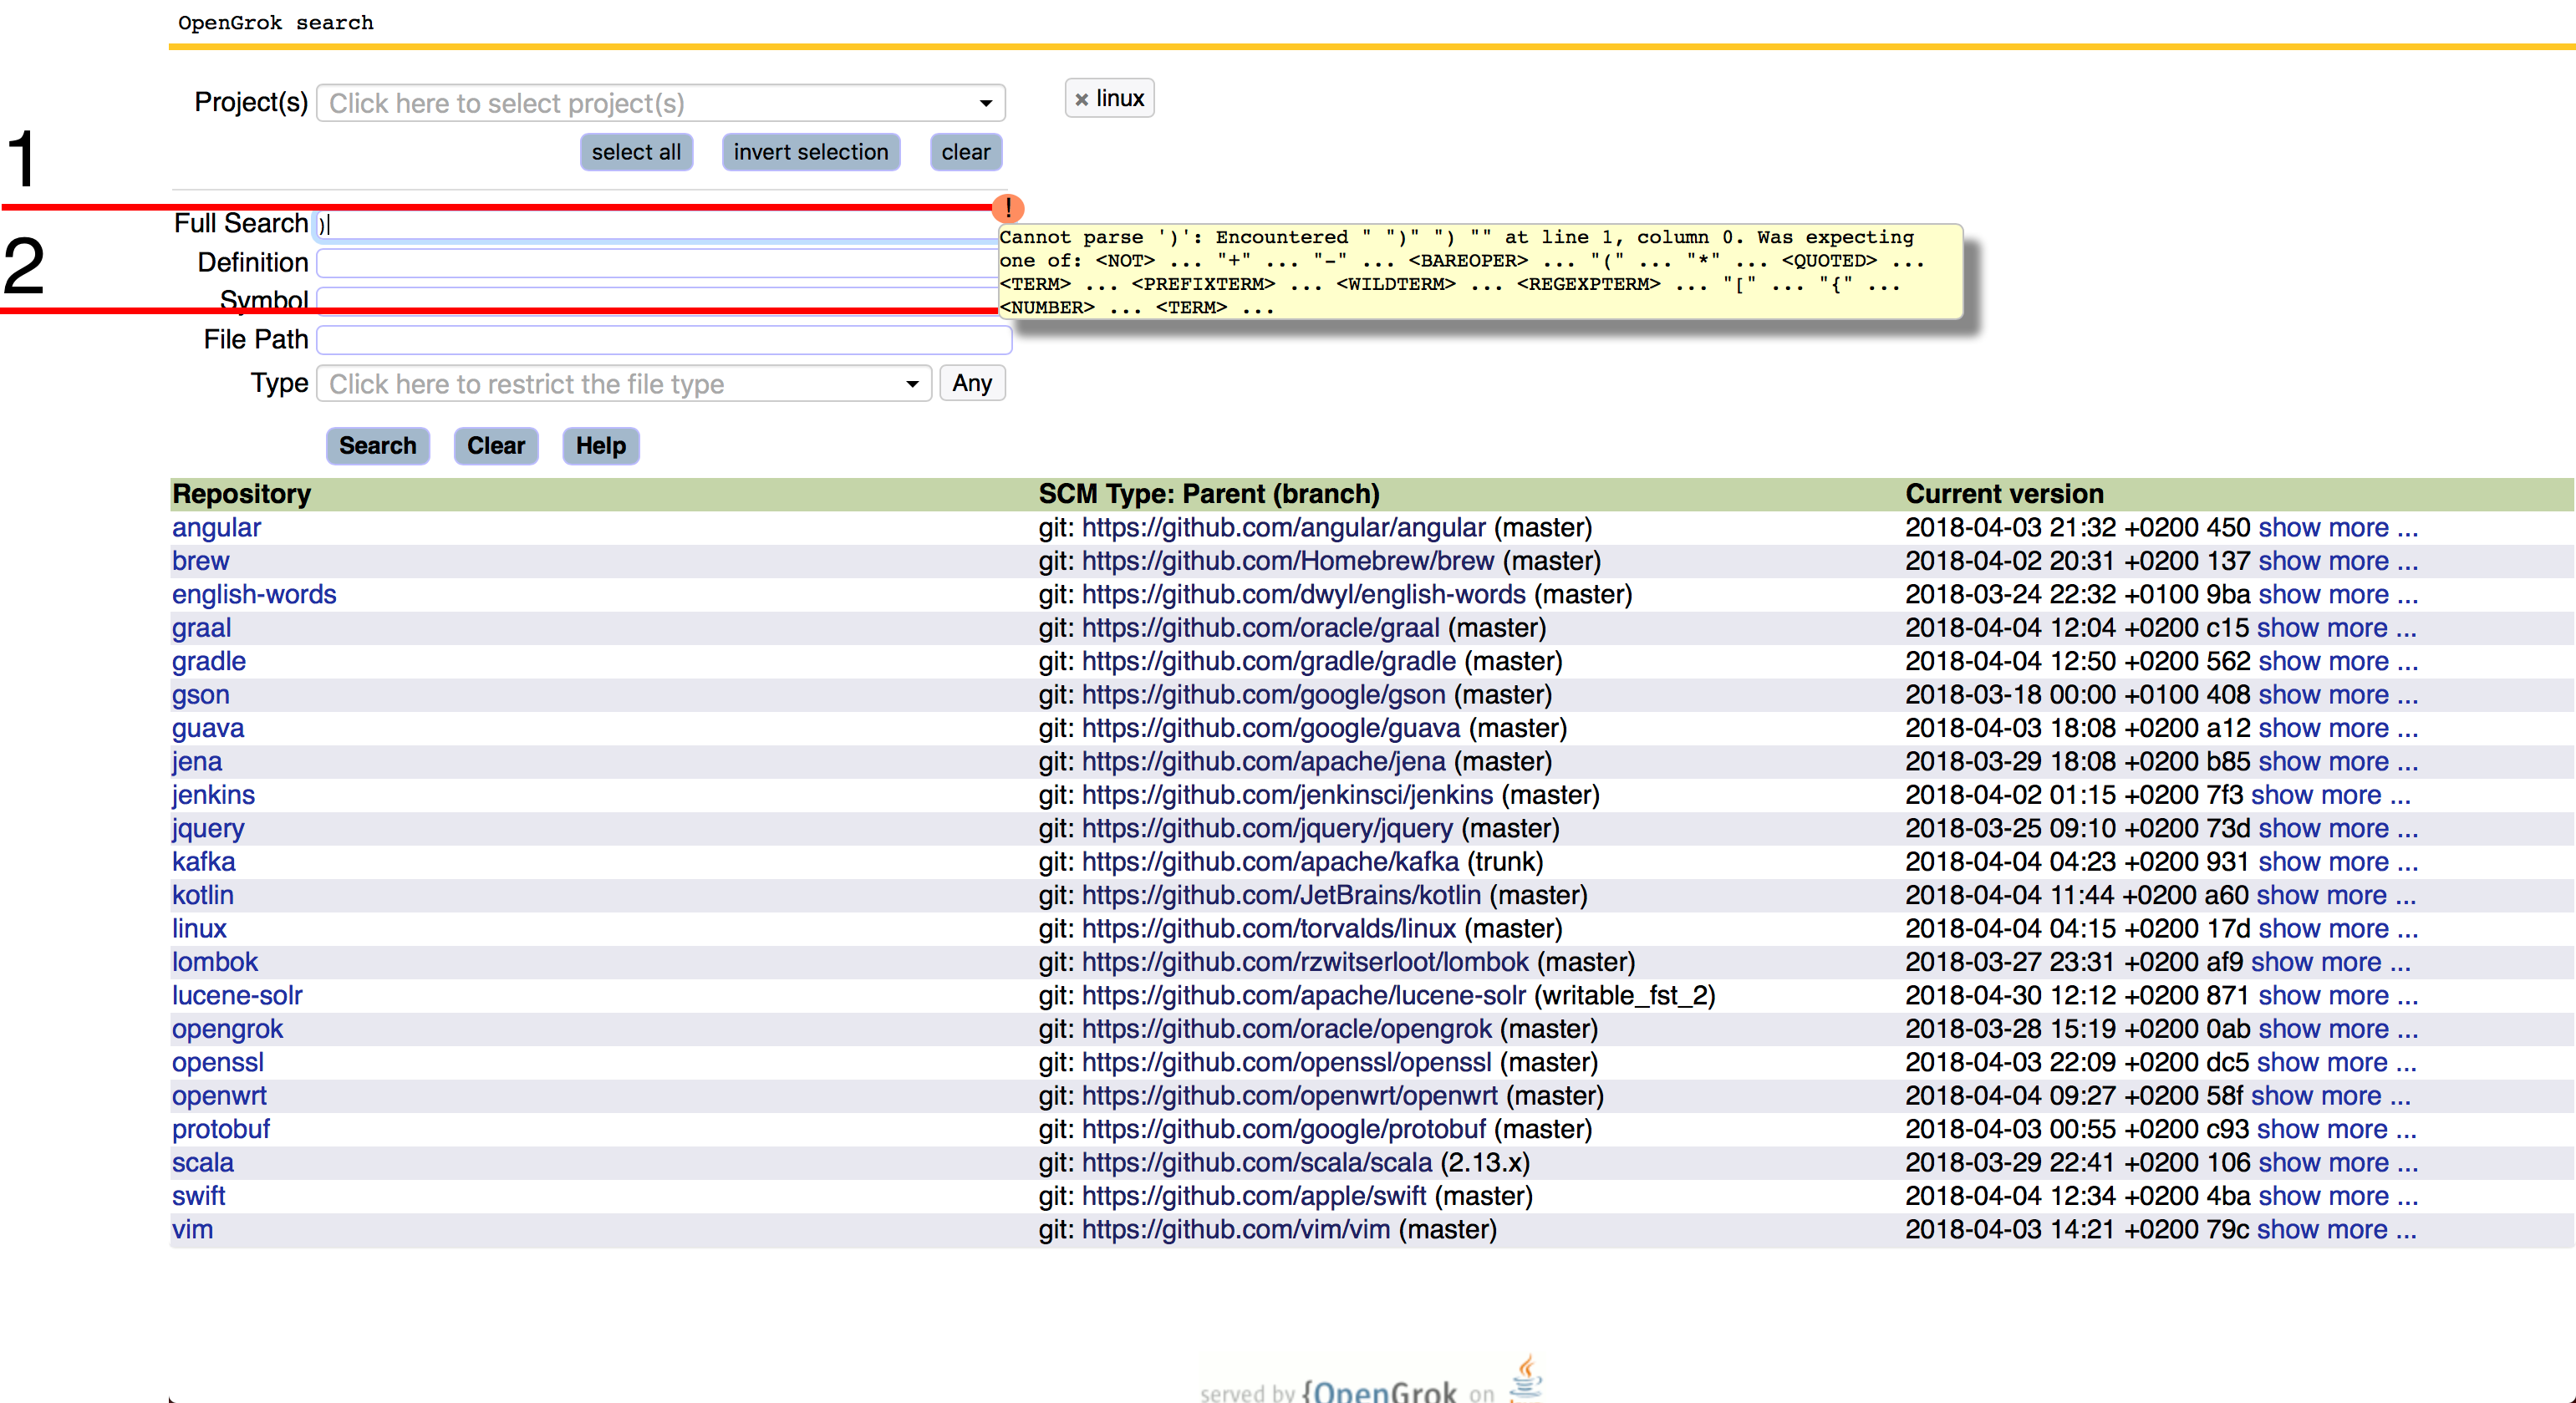
\includegraphics[width=145mm]{../img/suggestions_error.png}
    \caption{Suggestions error}
    \label{suggestions_error}
\end{figure}

The numbers in the figure \ref{suggestions_error} represent:
\begin{enumerate}
    \item Error notification.
    \item Detail of the error. This is only shown if the user hovers over the error notification.
\end{enumerate}

\subsubsection{Minisearch}
While traversing a source code or history, a minisearch field is available in the navigation menu. It allows users
to search in the current project. The suggestions are enabled for it as well. The result can look like in the figure
\ref{suggestions_minisearch}.

\begin{figure}[htbp]
    \centering
    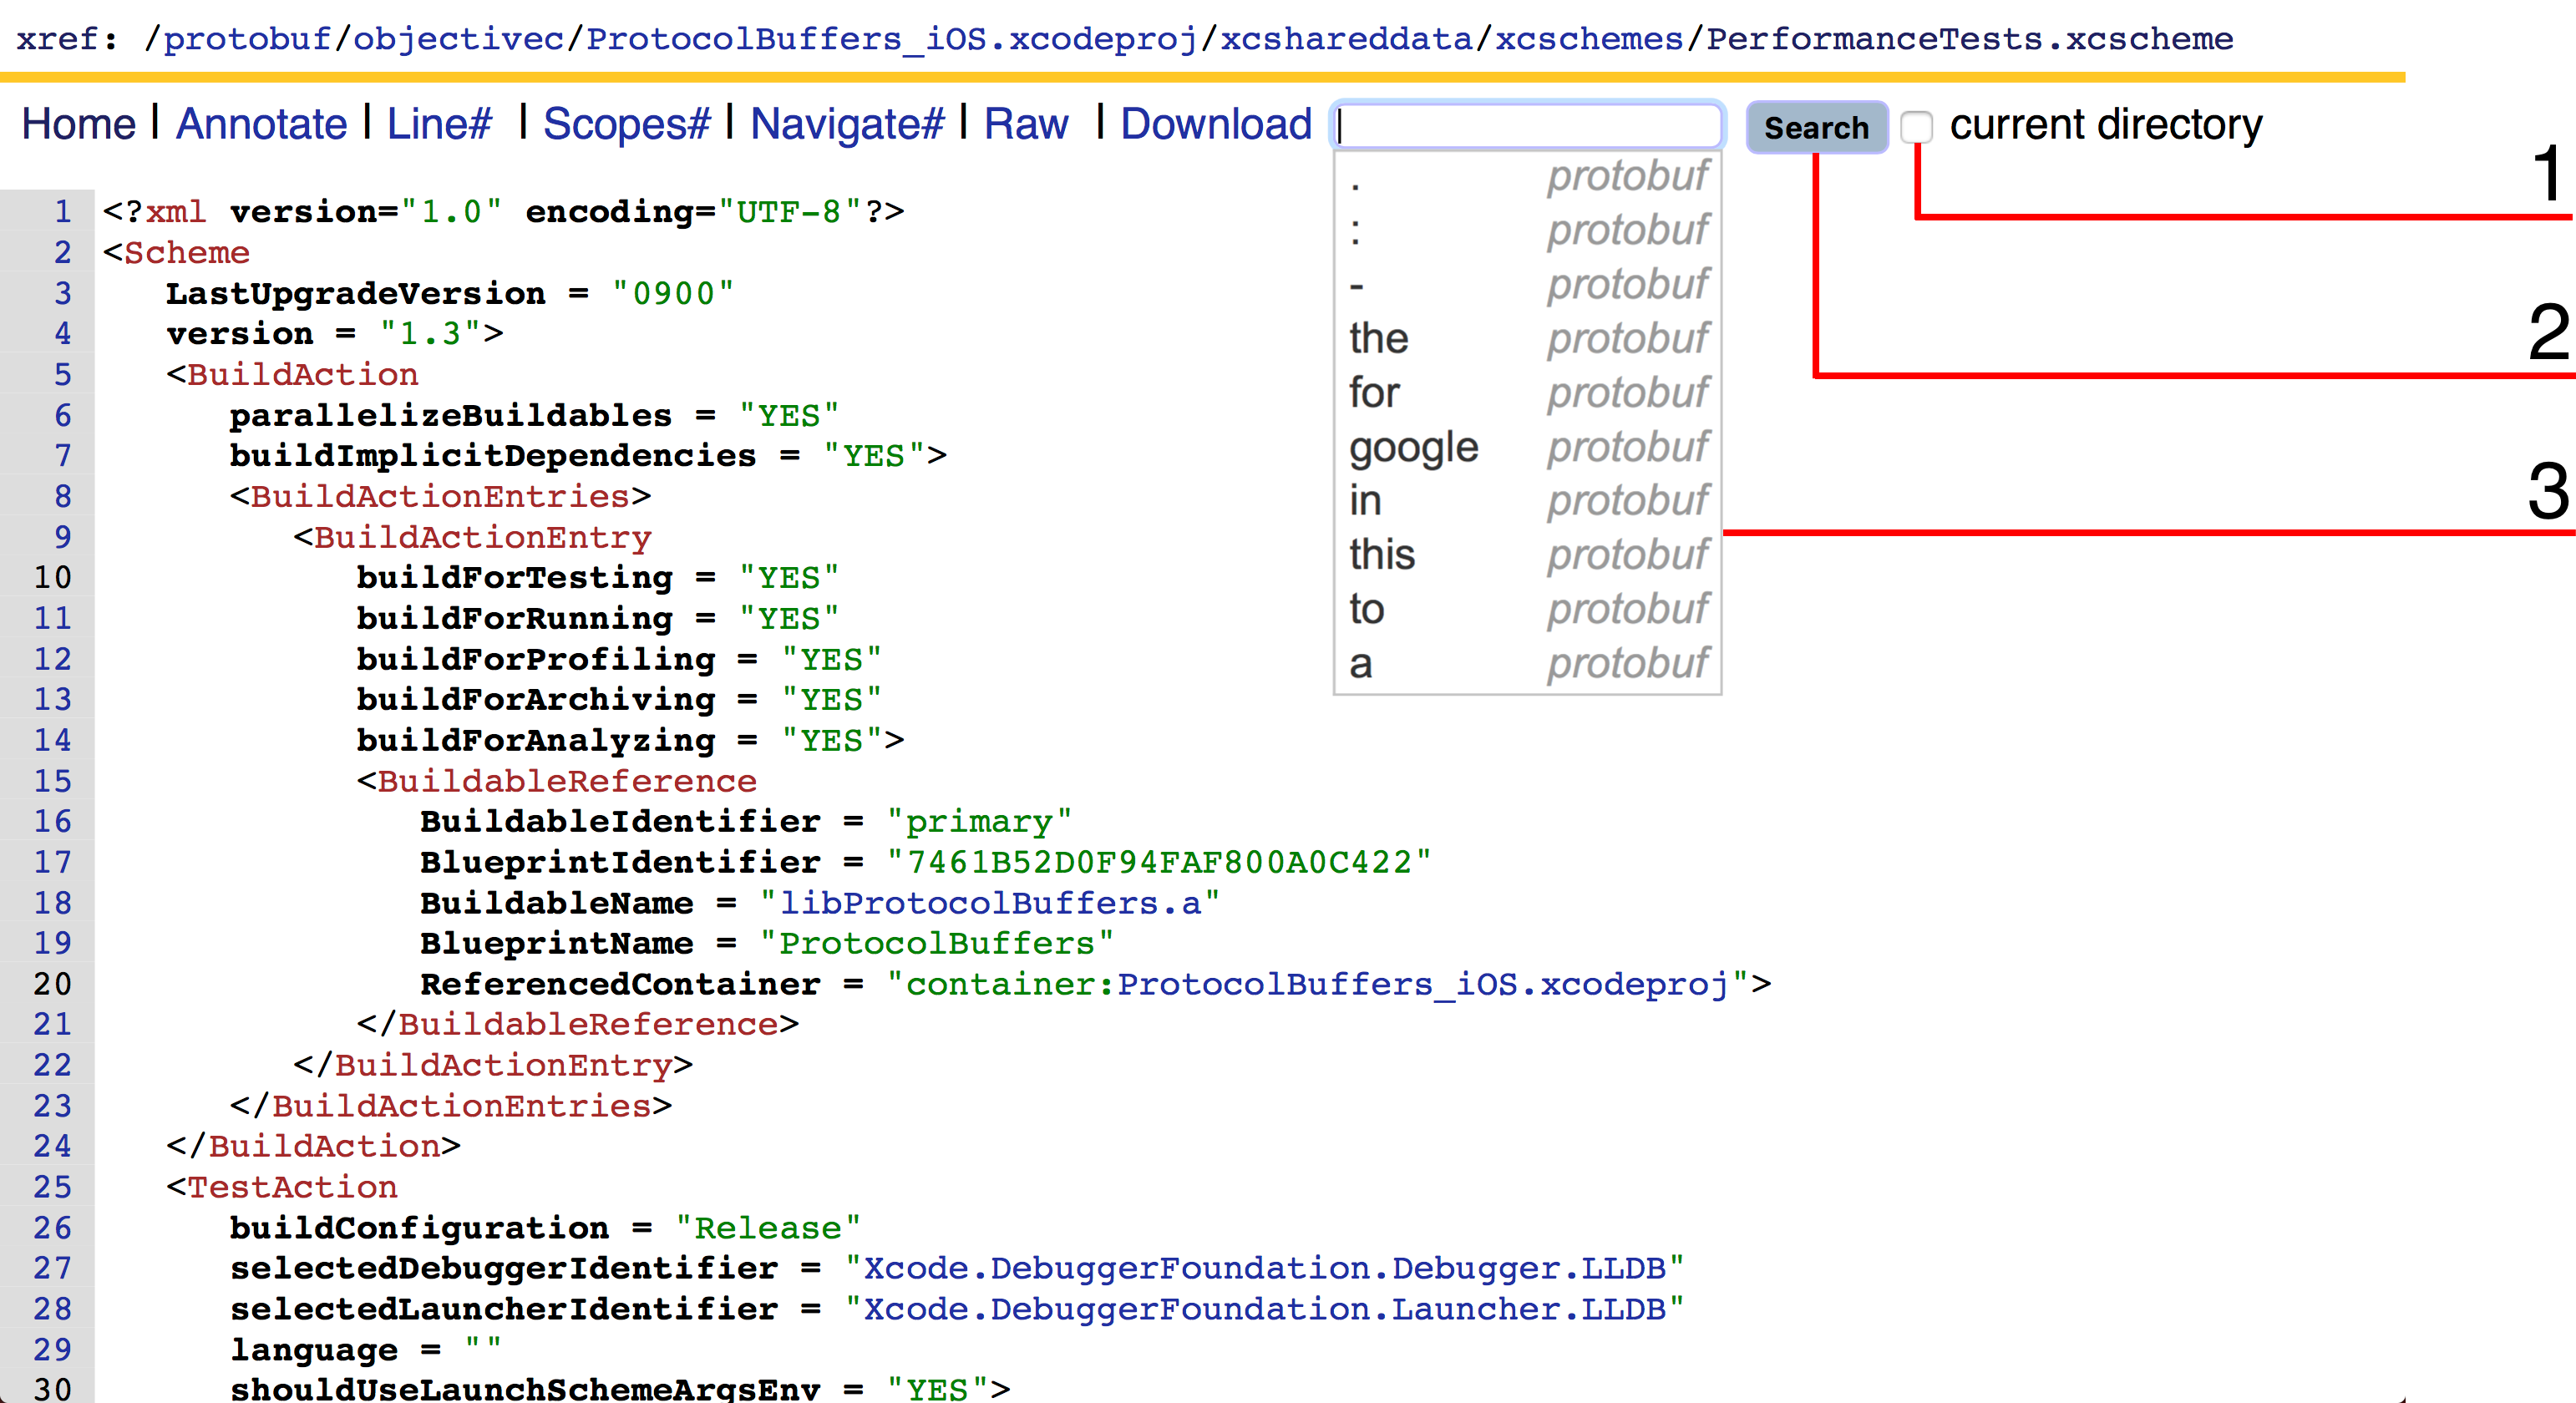
\includegraphics[width=145mm]{../img/minisearch.png}
    \caption{Suggestions for minisearch}
    \label{suggestions_minisearch}
\end{figure}

In the figure \ref{suggestions_minisearch} the numbers represent:
\begin{enumerate}
    \item The checkbox that specifies if the search (and consequently suggestions) should be restricted to the directory
    in which the displayed file is located. In this example it adds the following value to the \textit{path} field:
\begin{code}
"/protobuf/objectivec/ProtocolBuffers_iOS.xcodeproj/xcshareddata/xcschemes/"
\end{code}
    \item Search button that launches the search.
    \item Suggestions window as described before.
\end{enumerate}

\section{Administrator guide}
\label{administrator_guide}

There are multiple ways how to modify the suggester configuration described in \ref{suggester_config}:
\begin{itemize}
    \item By modifying the XML OpenGrok's configuration described in \ref{opengrok_configuration}. Example:
\begin{code}
<java version="1.8.0_162" class="java.beans.XMLDecoder">
  <object
      class="org.opensolaris.opengrok.configuration.Configuration"
      id="Configuration0">
    <void property="suggesterConfig">
      <void property="allowComplexQueries">
        <boolean>false</boolean>
      </void>
      <void property="allowMostPopular">
        <boolean>false</boolean>
      </void>
      <void property="allowedFields">
        <object class="java.util.Collections" method="singleton">
          <string>defs</string>
        </object>
      </void>
      <void property="allowedProjects">
        <object class="java.util.Collections" method="singleton">
          <string>fruitonserver</string>
        </object>
      </void>
      <void property="enabled">
        <boolean>false</boolean>
      </void>
      <void property="maxProjects">
        <int>2</int>
      </void>
      <void property="maxResults">
        <int>11</int>
      </void>
      <void property="minChars">
        <int>2</int>
      </void>
      <void property="rebuildCronConfig">
        <string>5 * * * *</string>
      </void>
      <void property="showProjects">
        <boolean>false</boolean>
      </void>
      <void property="showScores">
        <boolean>true</boolean>
      </void>
      <void property="showTime">
        <boolean>true</boolean>
      </void>
      <void property="suggesterBuildTerminationTimeSec">
        <int>500</int>
      </void>
    </void>
  </object>
</java>
\end{code}
    \item By using REST API configuration endpoint.
\end{itemize}
